% Created 2022-07-29 Fri 15:46
% Intended LaTeX compiler: xelatex
\documentclass[aspectratio=1610,xcolor={dvipsnames},hyperref={colorlinks,unicode,linkcolor=violet,anchorcolor=blueviolet,citecolor=YellowOrange,filecolor=black,urlcolor=Aquamarine}]{beamer}
\usepackage[dvipsnames]{xcolor}
\usepackage{graphicx}
\usepackage{grffile}
\usepackage{longtable}
\usepackage{booktabs}
\usepackage{wrapfig}
\usepackage{rotating}
\usepackage[normalem]{ulem}
\usepackage{amsmath}
\usepackage{textcomp}
\usepackage{amssymb}
\usepackage{capt-of}
\usepackage[colorlinks,unicode,linkcolor=violet,anchorcolor=blueviolet,citecolor=YellowOrange,filecolor=black,urlcolor=Aquamarine]{hyperref}
\usepackage{listings}
\usepackage{etoolbox}
\useoutertheme{infolines}
\setbeamertemplate{frametitle}{%
\usebeamerfont{frametitle}\insertframetitle\strut%
\vskip-0\baselineskip%
\leaders\vrule width .95\paperwidth\vskip1pt%
\vskip0pt%
\nointerlineskip
}

%% T for footer
\setbeamercolor{footlinecolor}{fg=cyan,bg=green}
\setbeamercolor{author in head/foot}{fg=blue}
\setbeamertemplate{footline}{%
\leavevmode%
\hbox{%
\begin{beamercolorbox}[wd=.26\paperwidth,ht=2.25ex,dp=1ex,left]{author in head/foot}%
\hspace*{2ex}\usebeamerfont{author in head/foot} Dept. CSE, UT Arlington
\end{beamercolorbox}%
\begin{beamercolorbox}[wd=.50\paperwidth,ht=2.25ex,dp=1ex,center]{author in head/foot}%
\usebeamerfont{title in head/foot}Scalable Modeling \& Imaging \& Learning Lab (SMILE)
\end{beamercolorbox}%
\begin{beamercolorbox}[wd=.24\paperwidth,ht=2.25ex,dp=1ex,right]{date in head/foot}%
\usebeamerfont{date in head/foot}
\insertshortdate{}\hspace*{1em}  % date
\insertframenumber/\inserttotalframenumber\hspace*{2ex}
\end{beamercolorbox}}%
\vskip0pt%
}
\usepackage{fontspec}
\usepackage[slantfont, boldfont]{xeCJK}
\setCJKmainfont{STFLGQKJF}
\usetheme{default}
\usefonttheme{serif}
\useinnertheme{circles}
\author{Nasy}
\date{Jul 29, 2022}
\title{Deep learning in Astronomy}
\hypersetup{
 pdfauthor={Nasy},
 pdftitle={Deep learning in Astronomy},
 pdfkeywords={},
 pdfsubject={},
 pdfcreator={Emacs 29.0.50 (Org mode 9.5.4)}, 
 pdflang={English}}
\usepackage[style=authortitle]{biblatex}
\addbibresource{~/.emacs.d/萚兮/旹/refs/ref.bib}
\begin{document}

\maketitle
\begin{frame}{Outline}
\tableofcontents
\end{frame}


\section{Introduction}
\label{sec:org32177cb}

\begin{frame}[label={sec:org955d099}]{Astronomy}
A branch of science that covers the study and analysis of all extraterrestrial objects and their phenomena.

\begin{itemize}
\item Origin
\item Evolution
\item Functions
\end{itemize}
\end{frame}

\begin{frame}[label={sec:orgfbee5af}]{Astronomy -- Method History}
\begin{itemize}
\item Observational astronomy (OA)
\begin{itemize}
\item Human eyes
\item Telescopes
\item Radio
\item Micrometer (e.g. double stars)
\item Spectrograph (e.g. redshift)
\item Photoelectric photometry using Charge-coupled Device (CCD), which
can record the image nearly down to the level of individual
photons.
\item Neutrino astronomy
\item Gravitational wave
\end{itemize}
\item Virtual observatory (VO)
\end{itemize}
\end{frame}

\begin{frame}[label={sec:orga81759b}]{Astronomy -- Fields}
Astronomy is divided into many subfields, such as galactic astronomy,
planetary science, extragalactic astronomy, stellar astronomy, solar
astronomy, and cosmology.  In general, the theoretical and the
observational.

The purpose of observational study is to observe, record, and collect
the data about the universe under study and theoretical scientists
mainly calculate the measurable consequences of physical models.

Theoretical astronomers use the collected data to generate the
simulation model, and the corresponding observations serve the purpose
of evaluating the model or indicating the need for tweaking them.
\end{frame}

\begin{frame}[label={sec:org38403e1}]{Astronomy -- Data}
With ultra-modern technology, the astronomical data collection has
been very simple, and rate is very high.  And in astronomy, there are
"4Vs" -- volume, variety, velocity, and value.

\begin{description}
\item[{Volume}] data size -- can be PB, EB, ZB.
\item[{Variety}] complex elements  -- signals, images, videos, spectra,
time series, and simulations.
\item[{Velocity}] rate of production and transmission -- sizeable synoptic
survey telescopes (LSST) 20 TB per night for ten years.
\item[{Value}] high value to the astronomy of the data.
\end{description}
\end{frame}

\begin{frame}[label={sec:orga961a0f}]{Data -- Data type}
\begin{itemize}
\item One-dimensional information in the form of signals;
\item Two-dimensional information in images;
\begin{itemize}
\item multispectral (8-10) and hyperspectral (100+).
\item From electromagnetic (EM) emissions
\item Image data
\item Spectral data
\end{itemize}
\item Three-dimensional information in the video?;
\item Time series (GW).

\item[{Electromagnetic Spectrum}] From \(1\) Hz to \(10^{25}\) Hz,  From km to
atom size.
\end{itemize}
\end{frame}

\begin{frame}[label={sec:orgd165f2f}]{Tasks}
\begin{itemize}
\item Stellar Classification \autocite{jing-minNewStellarSpectral2020,chiuSearchingYoungStellar2021}
\begin{itemize}
\item Most potential applications
\item O, B, A, F, G, K, and M.  (O and M represent the hottest and coolest types)
\end{itemize}
\item Pulsar Detection and Recognition (Time series, intensity and time)
\item Star / galaxy separation/classification and information analysis \autocite{hausenMorpheusDeepLearning2020}
\begin{itemize}
\item Shape and size
\end{itemize}
\item Transient Analysis (暂现源, Fast ratio burst (FRB), gamma-ray burst,
pulsar, gravitational
wave\autocite{zhangDetectingGravitationalWaves2022}, and other
transient phenomena)(FAST)
\item Astronomical survey analysis (e.g. Gaia survey, Active Galactic Nuclei(AGN))
\item Other applications
\end{itemize}
\end{frame}

\section{Papers}
\label{sec:org8c0fb40}

\begin{frame}[label={sec:org169747f}]{Paper 1}
\begin{itemize}
\item Detecting gravitational waves from extreme mass ratio inspirals (EMRI)
using convolutional neural networks
\autocite{zhangDetectingGravitationalWaves2022}
\item By: Xue-Ting Zhang, Chris Messenger, Natalia Korsakova, Man Leong
Chan, Yi-Ming Hu, and Jing-dong Zhang
\end{itemize}
\end{frame}

\begin{frame}[label={sec:org8e76c44}]{Gravitational waves}
\begin{itemize}
\item Double White Dwarfs (DWDs)
\item Massive Binary Black Holes (MBBHs)
\item Stellar-mass Binary Black Holes (sBBHs)
\item Extreme mass ratio inspirals (EMRIs)
\item Stochastic gravitational-wave background (mHz frequency band)
\end{itemize}
\end{frame}

\begin{frame}[label={sec:orge48385b}]{Waveform models of EMRIs}
\begin{itemize}
\item Teukolsky-based waveform and Numerical Kludge (NK) waveform.
\item Analytic Kludge (AK) model, through post-Newtonian equations (max
4.5 now)
\item Augmented Analytic Kludge (AAK). Accuracy similar to NK with the
generating speed of AK
\end{itemize}
\end{frame}

\begin{frame}[label={sec:org845a116}]{The TianQin (天琴) mission}
Ground noise affects accuracy, and TianQin is in space and can
accurately detect gravitational waves.

\begin{figure}[htbp]
\centering
\includegraphics[height=5cm]{./p2.png}
\caption{An example EMRI signals compared with the sensitivity curve of TianQin. A total length of 3 months observation time is assumed. From \cite{zhangDetectingGravitationalWaves2022}}
\end{figure}
\end{frame}

\begin{frame}[label={sec:orgce4cef9}]{Data}
Two categories.  One can express the data \(d\) as the addition of
random Gaussian noise \(n\) and the GW signal \(h\).

\begin{itemize}
\item \(d(t) = h(t) + n(t)\), if signal is present
\item \(d(t) = n(t)\), if there is no signal.
\end{itemize}

\begin{figure}[htbp]
\centering
\includegraphics[height=4cm]{./p3.png}
\caption{An example of whitened data in channel I in comparison with signal hI alone. For this event, the SNR is set to be 50. We draw the reader’s attention to the difference in scale for the noise and the signal. From \cite{zhangDetectingGravitationalWaves2022}}
\end{figure}
\end{frame}

\begin{frame}[label={sec:org662735a}]{Model}
\begin{description}
\item[{Input}] Simulation data for TianQin, using AK and AKK.
\begin{itemize}
\item 7864320 seconds (three months)
\item 1/30 Hz
\item 262144 size
\end{itemize}
\end{description}

\begin{center}
\includegraphics[height=4cm]{./p4.png}
\end{center}
\end{frame}

\begin{frame}[label={sec:org9e4b260}]{Experiment and Results}
\(M\) is MBH mass, \(10^4, 10^7\);  \(\rho\) is Signal-to-Noise Ratio
(SNR); \(z\) is redshift.

\begin{center}
\includegraphics[height=6cm]{./p6.png}
\end{center}
\end{frame}

\begin{frame}[label={sec:orgcfa1932}]{Experiment and Results}
\begin{figure}[htbp]
\centering
\includegraphics[height=5cm]{./p7.png}
\caption{The ROC curve of the signals from testing groups 1-3 is shown with the blue, purple, and red lines, respectively. The blue line indicates the expected effectiveness for group 1, the parameters have identical distribution to the training data; for group 2, the distribution is drawn from an astrophysical model; for group 3, the distribution is the same as group 1 and the training data, but switched to the AAK waveform model. The 1-\(\sigma\) confidence intervals are indicated by the shaded regions.}
\end{figure}
\end{frame}

\begin{frame}[label={sec:orgbe48363}]{Experiment and Results}
\begin{figure}[htbp]
\centering
\includegraphics[height=5cm]{./p8.png}
\caption{The comparison of the CNN sensitivity over EMRIs with different parameters.The vertical axis is the TAP, while the horizontal axis is the single varying parameter. The 1-σ confidence intervals are indicated by the shaded regions. The 1-\(\sigma\) confidence intervals are indicated by the shaded regions.}
\end{figure}
\end{frame}

\begin{frame}[label={sec:orge91f678}]{Paper 2}
\begin{itemize}
\item Morpheus: A Deep Learning Framework for the Pixel-level Analysis of
Astronomical Image Data \autocite{hausenMorpheusDeepLearning2020}
\item By: Ryan Hausen and Brant E. Robertson.
\end{itemize}
\end{frame}

\begin{frame}[label={sec:org12b97c1}]{Target}
\begin{itemize}
\item Source detection,
\item Source segmentation,
\item Morphological classification
\end{itemize}
\end{frame}

\begin{frame}[label={sec:org205197a}]{Model}
A U-Net.
\begin{description}
\item[{Input}] astronomical FITS images
\item[{Output}] types -- spheroid, disk, irregular, point source/compact, and background.
\end{description}

\begin{center}
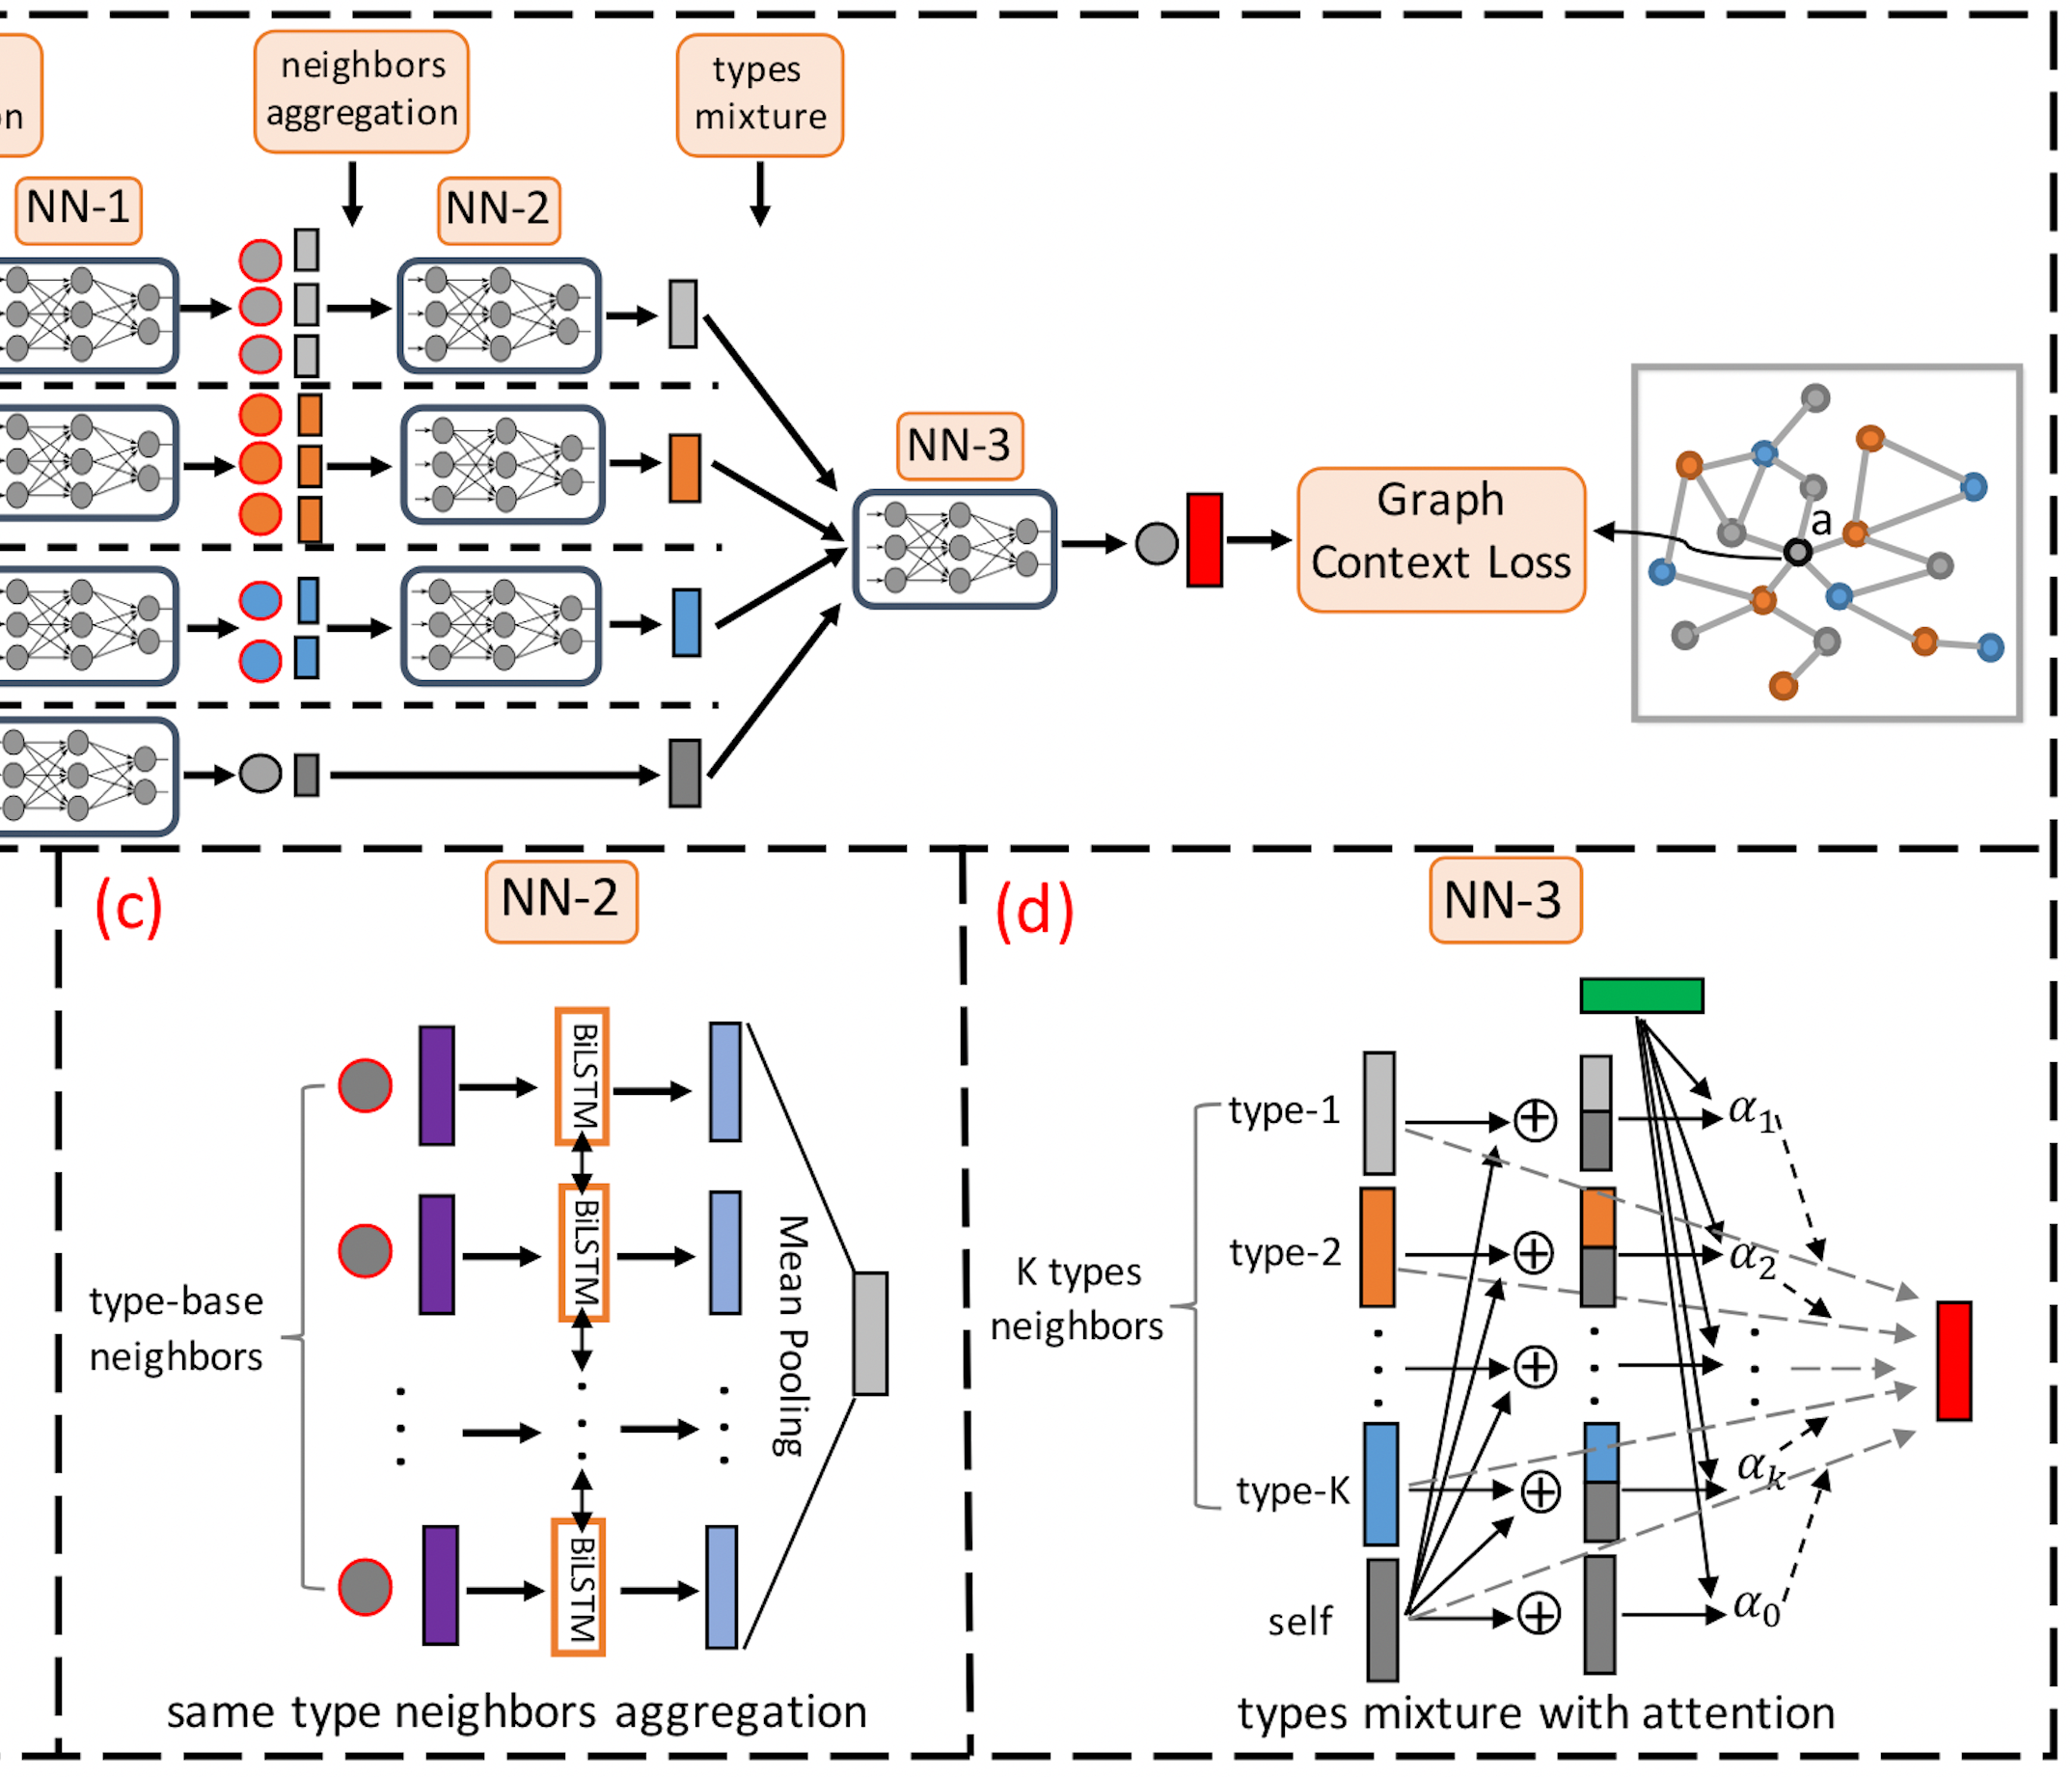
\includegraphics[width=.9\linewidth]{./p9.png}
\end{center}
\end{frame}

\begin{frame}[label={sec:org9c475be}]{Model -- Block}
\begin{figure}[htbp]
\centering
\includegraphics[height=5cm]{./p10.png}
\caption{A single block in the neural network architecture.  Panel (c) shows a single block from the architecture, parameterized by the number P (black) of block operations and the number Q (purple) of convolutional artificial neurons. Panel (b) shows an example zoom-in where there are P=2 groups of Q=4 block operations. Panel (a) shows a zoom-in on a block operation, which consists of batch normalization, Q = 4 CANs, and a rectified linear unit (ReLU).}
\end{figure}
\end{frame}

\begin{frame}[label={sec:org388f650}]{Classification results}
\begin{center}
\includegraphics[width=.9\linewidth]{./p11.png}
\end{center}
\end{frame}

\begin{frame}[label={sec:orge5644a2}]{Classification results}
\begin{columns}
\begin{column}{0.5\textwidth}

\begin{center}
\includegraphics[width=.9\linewidth]{./p12.png}
\end{center}

\end{column}
\begin{column}{0.5\textwidth}

\begin{center}
\includegraphics[width=.9\linewidth]{./p13.png}
\end{center}

\end{column}
\end{columns}
\end{frame}

\section{Refs}
\label{sec:orga25ba6e}

\begin{frame}[allowframebreaks]{Refs}
\printbibliography
\end{frame}
\end{document}